\subsection{Data Collection and Sources}
\label{sec:data_collection}

Our dataset comprises 1,247 blockchain security incidents collected from multiple sources spanning the period from January 2017 to December 2024. We employed a systematic approach to ensure comprehensive coverage while maintaining data quality and verifiability.

\subsubsection{Primary Data Sources}
We collected incident data from the following primary sources:
\begin{itemize}
    \item \textbf{Web3IsGoingGreat:} A comprehensive database of blockchain security incidents with detailed incident reports and loss estimates
    \item \textbf{Rekt News:} Specialized platform tracking DeFi exploits and protocol vulnerabilities
    \item \textbf{Secureum:} Academic and industry reports on smart contract vulnerabilities and attacks
    \item \textbf{Chainalysis:} Blockchain analytics data for incident verification and impact assessment
    \item \textbf{Academic Literature:} Peer-reviewed papers and technical reports from security conferences
\end{itemize}

\subsubsection{Inclusion and Exclusion Criteria}
To ensure data quality and relevance, we applied the following criteria:

\textbf{Inclusion Criteria:}
\begin{itemize}
    \item Minimum financial loss of \$10,000 USD (adjusted for inflation)
    \item Verifiable incident reports with multiple independent sources
    \item Clear attribution to specific blockchain platforms or protocols
    \item Sufficient technical details to classify the attack vector
\end{itemize}

\textbf{Exclusion Criteria:}
\begin{itemize}
    \item Purely anecdotal or unverified reports
    \item Incidents with insufficient technical details for classification
    \item Non-blockchain related security incidents
    \item Duplicate reports of the same incident
\end{itemize}

\subsubsection{Data Collection Protocol}
Our data collection process followed a standardized protocol:
\begin{enumerate}
    \item \textbf{Source Identification:} Systematic review of primary and secondary sources
    \item \textbf{Initial Screening:} Application of inclusion/exclusion criteria
    \item \textbf{Data Extraction:} Structured extraction of incident details, financial impact, and technical characteristics
    \item \textbf{Verification:} Cross-referencing with multiple sources for accuracy
    \item \textbf{Quality Control:} Review by multiple team members for consistency
\end{enumerate}

% TODO: Add specific details about date ranges, chains covered, and verification procedures

\begin{figure}[H]
\centering
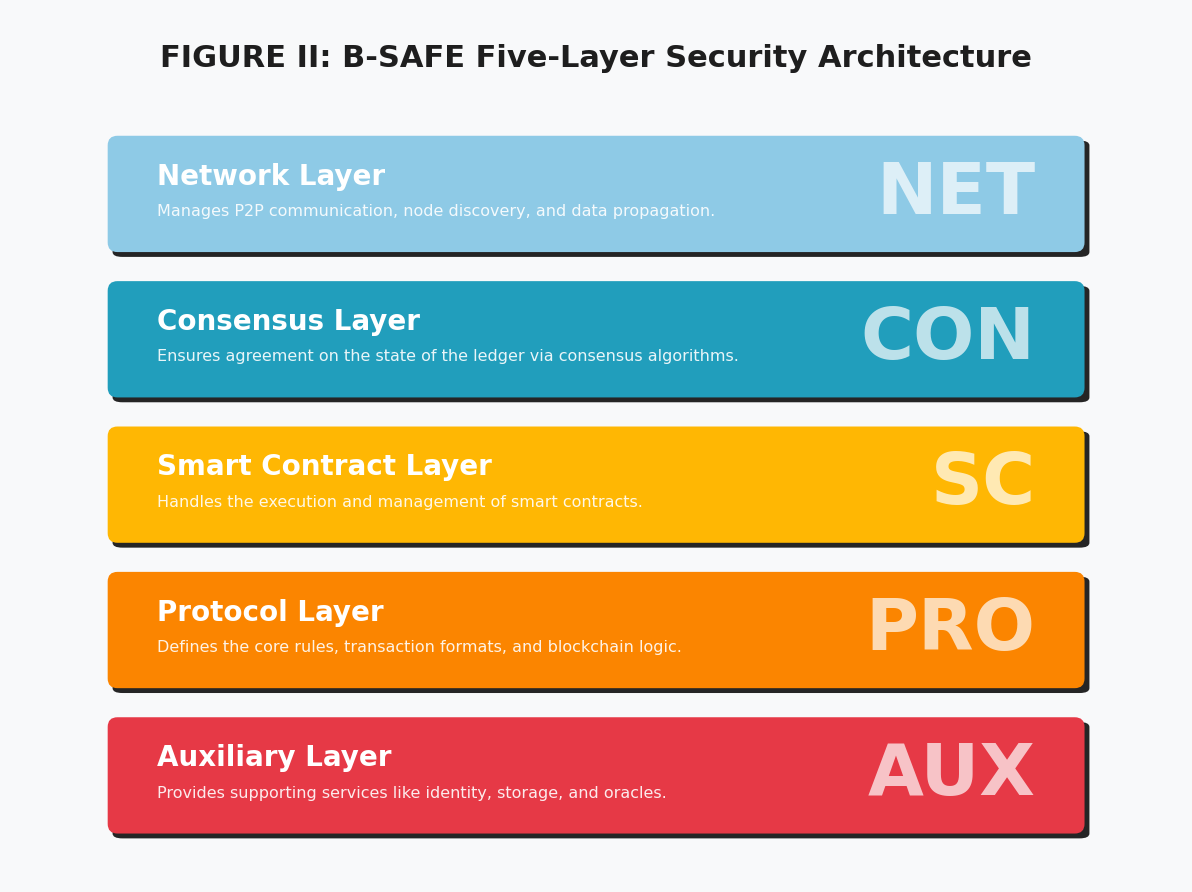
\includegraphics[width=0.4\textwidth]{../figure/fig2.png}
\caption{Systematic data collection and vetting pipeline ensuring data quality and reproducibility. The multi-stage process includes source identification, screening, extraction, verification, quality control, and labeling to produce a comprehensive and reliable dataset for analysis.}
\label{fig:data_pipeline}
\end{figure}
